% Source-faithful schematic redraw of the right triangular prism in printed question 27.
% The drawing is not to scale; no metric information is inferred from its shape.
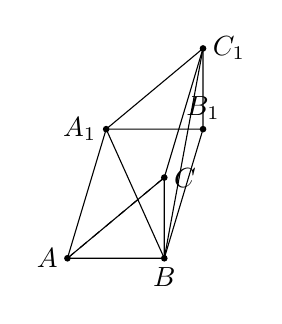
\begin{tikzpicture}[x=0.82cm,y=0.82cm,line cap=round,line join=round]
  \coordinate (A) at (-1.5,0);
  \coordinate (B) at (0,0);
  \coordinate (C) at (0,1.25);
  \coordinate (Aone) at (-0.9,2.0);
  \coordinate (Bone) at (0.6,2.0);
  \coordinate (Cone) at (0.6,3.25);

  % Prism edges; the long diagonal AC is hidden in the printed view.
  \draw[dashed] (A)--(C);
  \draw (A)--(B)--(C)--cycle;
  \draw (Aone)--(Bone)--(Cone)--cycle;
  \draw (A)--(Aone) (B)--(Bone) (C)--(Cone);
  % The plane through A_1, B, C_1 shown in the source diagram.
  \draw (Aone)--(B)--(Cone);

  \fill (A) circle (1.2pt) (B) circle (1.2pt) (C) circle (1.2pt)
        (Aone) circle (1.2pt) (Bone) circle (1.2pt) (Cone) circle (1.2pt);
  \node[left] at (A) {$A$};
  \node[below] at (B) {$B$};
  \node[right] at (C) {$C$};
  \node[left] at (Aone) {$A_1$};
  \node[above] at (Bone) {$B_1$};
  \node[right] at (Cone) {$C_1$};
\end{tikzpicture}
